% Karger's contraction algorithm on a small multigraph (generated by figs_c2ch08.py).
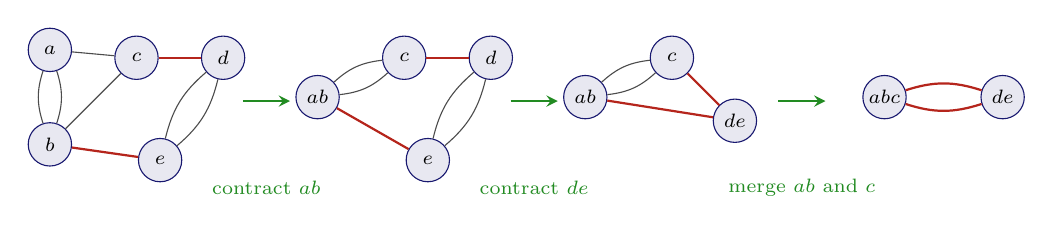
\begin{tikzpicture}[x=1cm,y=1cm,every node/.style={font=\small},>=stealth]
\tikzset{v/.style={circle,draw=MidnightBlue,fill=MidnightBlue!10,inner sep=1pt,minimum size=0.55cm,font=\scriptsize}}
\node[v] (p0a) at (0.0,1) {$a$};
\node[v] (p0b) at (0.0,-0.2) {$b$};
\node[v] (p0c) at (1.1,0.9) {$c$};
\node[v] (p0d) at (2.2,0.9) {$d$};
\node[v] (p0e) at (1.4,-0.4) {$e$};
\draw[black!70] (p0a) to[bend left=18] (p0b);
\draw[black!70] (p0a) to[bend right=18] (p0b);
\draw[black!70] (p0a) -- (p0c);
\draw[black!70] (p0b) -- (p0c);
\draw[BrickRed,thick] (p0c) -- (p0d);
\draw[BrickRed,thick] (p0b) -- (p0e);
\draw[black!70] (p0d) to[bend left=18] (p0e);
\draw[black!70] (p0d) to[bend right=18] (p0e);
\draw[->,thick,ForestGreen] (2.45,0.35) -- (3.05,0.35);
\node[font=\scriptsize,ForestGreen] at (2.75,-0.75) {contract $ab$};
\node[v] (p1ab) at (3.4,0.4) {$ab$};
\node[v] (p1c) at (4.5,0.9) {$c$};
\node[v] (p1d) at (5.6,0.9) {$d$};
\node[v] (p1e) at (4.8,-0.4) {$e$};
\draw[black!70] (p1ab) to[bend left=18] (p1c);
\draw[black!70] (p1ab) to[bend right=18] (p1c);
\draw[BrickRed,thick] (p1c) -- (p1d);
\draw[BrickRed,thick] (p1ab) -- (p1e);
\draw[black!70] (p1d) to[bend left=18] (p1e);
\draw[black!70] (p1d) to[bend right=18] (p1e);
\draw[->,thick,ForestGreen] (5.85,0.35) -- (6.449999999999999,0.35);
\node[font=\scriptsize,ForestGreen] at (6.15,-0.75) {contract $de$};
\node[v] (p2ab) at (6.8,0.4) {$ab$};
\node[v] (p2c) at (7.9,0.9) {$c$};
\node[v] (p2de) at (8.7,0.1) {$de$};
\draw[black!70] (p2ab) to[bend left=18] (p2c);
\draw[black!70] (p2ab) to[bend right=18] (p2c);
\draw[BrickRed,thick] (p2c) -- (p2de);
\draw[BrickRed,thick] (p2ab) -- (p2de);
\draw[->,thick,ForestGreen] (9.25,0.35) -- (9.85,0.35);
\node[font=\scriptsize,ForestGreen] at (9.55,-0.75) {merge $ab$ and $c$};
\node[v] (p3abc) at (10.6,0.4) {$abc$};
\node[v] (p3de) at (12.1,0.4) {$de$};
\draw[BrickRed,thick] (p3abc) to[bend left=18] (p3de);
\draw[BrickRed,thick] (p3abc) to[bend right=18] (p3de);
\end{tikzpicture}
